\documentclass[12pt]{article}
\usepackage{amsmath}
\usepackage{amssymb}
\usepackage{graphicx}
\usepackage{subcaption}
\usepackage{cite}
\usepackage{hyperref}
\usepackage{float}
\usepackage{xcolor}
\usepackage{listings}
\usepackage{minted}

\hypersetup{
    colorlinks=true,
    linkcolor=black,   % Color of internal links (e.g., toc, sections, etc.)
    citecolor=black,   % Color of citation links (e.g., bibliography)
    urlcolor=black     % Color of external links (e.g., URLs)
}

\title{Path Tracing Renderer Using Monte Carlo Methods}
\author{Silas Maughan}
\date{\today}

\begin{document}

\maketitle
\begin{abstract}
    This report presents an expository on the foundational mathematical knowledge and implementation of a path tracing renderer using Monte Carlo methods to simulate realistic lighting in a 3D scene. Various sampling techniques and variance reduction methods are explored to enhance image quality and convergence speed. Experimental results demonstrate the effectiveness of these techniques in reducing noise and improving rendering efficiency.
\end{abstract}

\tableofcontents
\break
\section{Introduction}
\label{sec:intro}
\subsection{Purpose and Scope}
\subsubsection{Goals of the Document}

This expository aims to achieve the following objectives:
\begin{enumerate}
    \item To provide a comprehensive analysis of the \textit{mathematical} foundations underlying path tracing, creating a scene, and Monte Carlo integration techniques.

    \item To demonstrate the \textit{visual} impact of Monte Carlo methods in path tracing for realistic light simulation, exploring their impact on image fidelity, convergence rates, and rendering efficiency.

    \item To elucidate the \textit{design} and implementation of a path tracing system, with particular emphasis on acceleration structures like Bounding Volume Hierarchies (BVH), real-time visualisation with OpenGL and adhering to software modelling principles.
\end{enumerate}

Through these objectives, this document seeks to offer a thorough exploration of path tracing, from its mathematical underpinnings to its practical realization in computer graphics, serving as a valuable resource for researchers and practitioners in the field of physically-based rendering.

\subsubsection{Overview of the Methodological Approach}
This expository adopts a progressive approach to the principles and implementation of path tracing.
We begin by examining the foundational elements of a generic path tracer, including ray representation, intersection testing, and basic shading models. For each of these components, we present the underlying mathematical principles, followed by their corresponding code implementations. This foundational phase establishes the core concepts upon which more advanced techniques are built.

Building upon these foundational elements, we then abstract the entire lighting simulation process into a comprehensive mathematical framework. This transition allows us to view the path tracing problem as an integration task. We introduce Monte Carlo methods as a powerful tool for numerical integration, exploring how these statistical techniques can be applied to solve the rendering equation efficiently.

As we introduce each component, we demonstrate its effect on the rendered image, allowing for a clear understanding of how theoretical concepts translate to visual outcomes. This iterative approach provides immediate feedback on the impact of each implemented feature, reinforcing the connection between mathematical principles and their applications in computer graphics.

\subsection{Background}
\subsubsection{Overview of Ray Tracing}
Ray tracing is a rendering technique that simulates the physical behavior of light to create realistic images. At its core, ray tracing involves tracing the path of light rays as they interact with objects in a virtual scene \cite{Glassner1989}.
The fundamental concept is to cast rays from a virtual camera through each pixel of an image plane into the scene. These rays interact with objects, potentially reflecting, refracting, or being absorbed, mimicking the behavior of light in the real world. By accurately modeling these interactions, ray tracing can produce highly realistic effects such as shadows, reflections, and refractions.

Path tracing, an advanced form of ray tracing, extends this concept by using Monte Carlo methods to solve the rendering equation \cite{Kajiya1986}. It traces numerous light paths through the scene, accounting for multiple bounces and complex light interactions. This approach allows for the accurate simulation of global illumination effects, including soft shadows, color bleeding, and caustics \cite{Veach1997}.

The power of ray tracing and path tracing lies in their ability to naturally handle a wide range of lighting phenomena, producing physically accurate images. However, this accuracy comes at the cost of increased computational complexity, often requiring sophisticated optimization techniques to achieve reasonable rendering times \cite{Pharr2016}.
\subsubsection{Importance in Computer Graphics}
Path tracing has become a cornerstone technique in modern computer graphics, particularly in applications demanding high levels of photorealism. Its ability to accurately simulate complex light interactions makes it invaluable in industries such as film and television visual effects, architectural visualization, product design, and video game development \cite{Keller2015}.

In the film industry, path tracing is used to create photorealistic CGI that seamlessly blends with live-action footage \cite{Christensen2018}. Moreover, with the advent of real-time ray tracing in consumer hardware, path tracing techniques are increasingly being adopted in interactive applications like video games, pushing the boundaries of real-time graphics fidelity \cite{Schied2017}.
\section{Ray Tracing Fundamentals}
\label{sec:fundamentals}

\subsection{Rays}
\subsubsection{A Ray of Light as a Vector}
In physics, light is an electromagnetic wave that propagates through space. However, in many scenarios, particularly in computer graphics, we can approximate light behavior using the concept of rays. This simplification, known as geometric optics, is valid when the wavelength of light is much smaller than the objects it interacts with.

A ray of light can be thought of as an idealized narrow beam of light traveling in a straight line. This approximation allows us to model light propagation without dealing with the complexities of wave optics, making it computationally feasible for rendering purposes.

In mathematics, a vector is a quantity that has both magnitude and direction. It can be represented as an arrow in space, defined by its starting point and its direction. This concept aligns perfectly with our need to represent a ray of light, which has a point of origin and a direction of propagation.

Formally, we can define a ray \(\mathbf{R}(t)\) in 3D space using a parametric equation:

\[
    \mathbf{R}(t) = \mathbf{O} + t\mathbf{D}
\]

where:
\begin{itemize}
    \item \(\mathbf{O}\) is the origin point of the ray (a 3D vector)
    \item \(\mathbf{D}\) is the direction vector of the ray (a 3D unit vector)
    \item \(t\) is a scalar parameter (\(t \geq 0\))
\end{itemize}

This equation describes all points along the ray, starting from the origin and extending infinitely in the direction of \(\mathbf{D}\). In practice, we often constrain \(t\) to an interval \([t{\text{min}}, t{\text{max}}]\) to define a specific segment of the ray.

\subsection{Intersection Testing}

Having established the mathematical and programmatic representation of a ray of light, we now turn our attention to determining how these rays interact with objects in our scene. Intersection testing is a crucial component of ray tracing, allowing us to simulate the behavior of light as it encounters various surfaces. To perform these tests efficiently, we leverage the geometric properties of vectors.

\subsubsection{Mathematical Tools}

Two fundamental vector operations are essential for intersection testing: the dot product and the cross product.

\paragraph{Dot Product}
The dot product of two vectors \(\mathbf{A}\) and \(\mathbf{B}\) is a scalar quantity defined as:
\[
    \mathbf{A} \cdot \mathbf{B} = Ax Bx + Ay By + Az Bz
\]

This operation has several useful properties for intersection testing:

\begin{itemize}
    \item It can be used to calculate the angle between two vectors:
          \[
              \cos(\theta) = \frac{\mathbf{A} \cdot \mathbf{B}}{\|\mathbf{A}\| \|\mathbf{B}\|}
          \]
    \item It allows us to determine orthogonality (when the dot product is zero)
    \item It enables the computation of vector projections
\end{itemize}

In the context of ray tracing, the dot product is particularly useful for determining the angle between a ray and a surface normal, which is crucial for calculating reflection and refraction.

\paragraph{Cross Product}
The cross product of two vectors \(\mathbf{A}\) and \(\mathbf{B}\) results in a third vector \(\mathbf{C}\) that is perpendicular to both:
\[
    \mathbf{C} = \mathbf{A} \times \mathbf{B} = \left( Ay Bz - Az By, Az Bx - Ax Bz, Ax By - Ay Bx \right)
\]

The magnitude of the resulting vector is given by:
\[
    \|\mathbf{C}\| = \|\mathbf{A}\| \|\mathbf{B}\| \sin(\theta)
\]
where \(\theta\) is the angle between \(\mathbf{A}\) and \(\mathbf{B}\).

In intersection testing, the cross product serves several important purposes:

\begin{itemize}
    \item It can be used to compute surface normals for triangles or polygons
    \item It helps in determining the orientation of surfaces relative to the ray
    \item It's useful in calculating barycentric coordinates for triangle intersection tests
    \item It can be employed to find perpendicular vectors, which is helpful in constructing coordinate systems for shading calculations
\end{itemize}

These mathematical tools form the foundation for implementing various intersection tests. For instance, when testing ray-triangle intersections, we can use the cross product to compute the triangle's normal and the dot product to determine if the ray is facing the correct side of the triangle. Similarly, for ray-plane intersections, the dot product helps us calculate the distance along the ray at which the intersection occurs.

In the following sections, we will explore how these tools are applied to specific geometric primitives, starting with spheres and planes, and then extending to more complex shapes and acceleration structures. By leveraging these vector operations, we can efficiently determine not only if a ray intersects an object, but also the exact point of intersection and the surface properties at that point, which are crucial for accurate light transport simulation in our path tracer.

\subsubsection{Spheres}

A sphere is a common geometric object in ray tracing, defined by its center \(\mathbf{C}\) and radius \(R\). To determine the intersection of a ray with a sphere, we substitute the ray equation \(\mathbf{P}(t) = \mathbf{O} + t\mathbf{D}\) into the sphere's implicit equation:
\[
    \left\| \mathbf{P}(t) - \mathbf{C} \right\|^2 = R^2
\]
Expanding and simplifying this equation yields:
\[
    \left\| \mathbf{O} + t\mathbf{D} - \mathbf{C} \right\|^2 = R^2
\]
\[
    \left( \mathbf{O} - \mathbf{C} + t\mathbf{D} \right) \cdot \left( \mathbf{O} - \mathbf{C} + t\mathbf{D} \right) = R^2
\]
\[
    (\mathbf{O} - \mathbf{C}) \cdot (\mathbf{O} - \mathbf{C}) + 2t \left( \mathbf{O} - \mathbf{C} \right) \cdot \mathbf{D} + t^2 \mathbf{D} \cdot \mathbf{D} = R^2
\]
This is a quadratic equation in \(t\):
\[
    t^2 \mathbf{D} \cdot \mathbf{D} + 2t \left( \mathbf{O} - \mathbf{C} \right) \cdot \mathbf{D} + \left( (\mathbf{O} - \mathbf{C}) \cdot (\mathbf{O} - \mathbf{C}) - R^2 \right) = 0
\]
Letting \(\mathbf{L} = \mathbf{O} - \mathbf{C}\), \(a = \mathbf{D} \cdot \mathbf{D}\), \(b = 2 \mathbf{L} \cdot \mathbf{D}\), and \(c = \mathbf{L} \cdot \mathbf{L} - R^2\), we solve the quadratic equation:
\[
    at^2 + bt + c = 0
\]
The solutions for \(t\) are given by:
\[
    t = \frac{-b \pm \sqrt{b^2 - 4ac}}{2a}
\]
The discriminant \(b^2 - 4ac\) determines the nature of the intersection:
\begin{itemize}
    \item If \(b^2 - 4ac < 0\), the ray does not intersect the sphere.
    \item If \(b^2 - 4ac = 0\), the ray tangentially intersects the sphere at one point.
    \item If \(b^2 - 4ac > 0\), the ray intersects the sphere at two points.
\end{itemize}

The following image illustrates a ray-sphere intersection:

\begin{figure}[H]
    \centering
    
\includegraphics[width=0.5\textwidth]{images/intersections/ray_sphere_intersection.png}
    \caption{Ray-sphere intersection demonstration}
    \label{fig:raysphereintersection}
\end{figure}

In Figure \ref{fig:raysphereintersection}, we can see a red circle representing a sphere on a white background. Notice the jagged pixelated border. This is because at one ray per pixel, a pixel can only be fully red (intersecting the sphere) or fully white (missing the sphere). We will fix this issue later.

\subsubsection{Planes}

A plane is defined by a point \(\mathbf{P}_0\) on the plane and a normal vector \(\mathbf{N}\). To find the intersection of a ray with a plane, we use the plane equation:
\[
    \mathbf{N} \cdot \left( \mathbf{P}(t) - \mathbf{P}_0 \right) = 0
\]
Substituting the ray equation \(\mathbf{P}(t) = \mathbf{O} + t\mathbf{D}\):
\[
    \mathbf{N} \cdot \left( \mathbf{O} + t\mathbf{D} - \mathbf{P}_0 \right) = 0
\]
\[
    \mathbf{N} \cdot \mathbf{O} + t \left( \mathbf{N} \cdot \mathbf{D} \right) - \mathbf{N} \cdot \mathbf{P}_0 = 0
\]
Solving for \(t\):
\[
    t = \frac{\mathbf{N} \cdot (\mathbf{P}_0 - \mathbf{O})}{\mathbf{N} \cdot \mathbf{D}}
\]
provided \(\mathbf{N} \cdot \mathbf{D} \neq 0\). If \(\mathbf{N} \cdot \mathbf{D} = 0\), the ray is parallel to the plane and does not intersect it.

The following image illustrates a ray-plane intersection:

\begin{figure}[H]
    \centering
    
\includegraphics[width=0.5\textwidth]{images/intersections/ray_quad_intersection.png}
    \caption{Ray-plane intersection demonstration}
    \label{fig:rayplaneintersection}
\end{figure}

In Figure \ref{fig:rayplaneintersection}, we can see a ray intersecting a plane (represented as a quad for visualization purposes). The image demonstrates how a ray intersects the plane at a single point. This visual representation helps to understand the mathematical concept described above, where we solve for a single value of \(t\) to find the intersection point.

\subsubsection{Extension to Object Meshes}

Intersection tests can be extended to complex object meshes using triangle intersection algorithms. This is a crucial step in ray tracing, as most 3D models are represented as meshes composed of triangles.

\paragraph{Triangle Intersection}

UNNECESSARY TO DEMONSTRATE, REMOVE OR IMPROVE


The most common method for triangle intersection is the Möller–Trumbore algorithm. This algorithm is efficient and doesn't require precomputation of the triangle plane equation.

Given a ray \(\mathbf{R}(t) = \mathbf{O} + t\mathbf{D}\) and a triangle defined by vertices \(\mathbf{V}0\), \(\mathbf{V}1\), and \(\mathbf{V}_2\), we can express any point on the triangle as:

\[
    \mathbf{T}(u,v) = (1-u-v)\mathbf{V}0 + u\mathbf{V}1 + v\mathbf{V}_2
\]

where \(u\) and \(v\) are barycentric coordinates satisfying \(u \geq 0\), \(v \geq 0\), and \(u + v \leq 1\).

The intersection point must satisfy:

\[
    \mathbf{O} + t\mathbf{D} = (1-u-v)\mathbf{V}0 + u\mathbf{V}1 + v\mathbf{V}_2
\]

This can be rewritten as a system of linear equations:

\[
    \begin{bmatrix}
        -\mathbf{D} & \mathbf{V}1 - \mathbf{V}0 & \mathbf{V}2 - \mathbf{V}0
    \end{bmatrix}
    \begin{bmatrix}
        t \\ u \\ v
    \end{bmatrix}
    = \mathbf{O} - \mathbf{V}_0
\]

Solving this system using Cramer's rule gives us \(t\), \(u\), and \(v\). If \(0 \leq u \leq 1\), \(0 \leq v \leq 1\), \(u + v \leq 1\), and \(t > 0\), then the ray intersects the triangle.

\paragraph{Mesh Intersection}

For a mesh composed of many triangles, we perform the following steps:

For each triangle in the mesh:
a. Perform the triangle intersection test.
b. If an intersection is found, store the intersection point and distance.

After testing all triangles, return the closest intersection point (smallest positive \(t\)).

\subsection{Placing Objects into the World}

In computer graphics, assembling a scene involves not only defining the objects within it but also positioning them appropriately. Consider the classic demonstration scene known as the \textit{Cornell Box}~\cite{cornellbox}, which is a standard test for rendering algorithms to showcase accurate light transport and shading.
From the previous sections, we've discussed how to test intersections with various geometric primitives. However, to build a complex scene like the Cornell Box, we need a systematic way to place and manipulate these objects in three-dimensional space.

Matrices are fundamental tools in linear algebra that we can use to efficiently represent and compute transformations in space. We can represent operations such as:

\begin{itemize}
    \item \textbf{Translation} moves an object by a certain distance along the axes.
    \item \textbf{Rotation} turns an object around an axis passing through the origin.
    \item \textbf{Scaling} resizes an object by stretching or compressing it along the axes.
\end{itemize}

and put them all into mathematical objects that can be easily combined and applied to points and vectors in 3D space (and computed quickly on a GPU).

In our path tracer we can view a point or vector as a column vector (a matrix of N $\times$ 1):
\[
    \mathbf{v} = \begin{pmatrix} x \\ y \\ z \end{pmatrix}
\]
Transforming this vector involves multiplying it by a transformation matrix:
\[
    \mathbf{v}' = \mathbf{M} \mathbf{v}
\]
where \(\mathbf{v}'\) is the transformed vector and \(\mathbf{M}\) is the transformation matrix.
If this transformation matrix is then applied to all points in our object, then we have successfully transformed our object.

\subsubsection{Translation}

We will start with translation as though it may appear the most simple:
\( \mathbf{v}' = \mathbf{v} + \mathbf{d} \)
where \( \mathbf{d} = \begin{bmatrix} dx \\ dy \\ dz \end{bmatrix} \) is the translation vector.
Unfortunately, this breaks the laws of linearity (see \autoref{sec:appendix-derivations-linear}).

This is a problem because translation cannot be represented with a 3$\times$3 matrix in 3D space.


To unify translation with rotation and scaling in a single matrix operation, we introduce homogeneous coordinates. By adding an extra dimension to our vectors and matrices, we can represent all affine transformations, including translation, with 4$\times$4 matrices.

In homogeneous coordinates, a point becomes:

\[
    \mathbf{v}_h = \begin{pmatrix} x \\ y \\ z \\ 1 \end{pmatrix}
\]

A translation matrix in homogeneous coordinates is:

\[
    \mathbf{T} = \begin{pmatrix}
        1 & 0 & 0 & d_x \\
        0 & 1 & 0 & d_y \\
        0 & 0 & 1 & d_z \\
        0 & 0 & 0 & 1   \\
    \end{pmatrix}
\]

The transformation is then applied via:

\[
    \begin{bmatrix}  1 & 0 & 0 & {T_x} \\ 0 & 1 & 0 & {T_y} \\ 0 & 0 & 1 & {T_z} \\ 0 & 0 & 0 & 1 \end{bmatrix} \cdot \begin{pmatrix} x \\ y \\ z \\ 1 \end{pmatrix} = \begin{pmatrix} x + {T_x} \\ y + {T_y} \\ z + {T_z} \\ 1 \end{pmatrix}
\]



While we primarily use 3$\times$3 matrices for rotation and scaling in our renderer, working with homogeneous coordinates and 4$\times$4 matrices becomes essential for incorporating translation and perspective transformations, especially in more advanced rendering techniques.

\subsubsection{Scaling}

Scaling \textit{is} a linear transformation which means that it can be represented using a 3$\times$3 matrix, however as we would like all our transformations to multiply with each other we add a 4th scaling value of 1.

\[
    \begin{bmatrix}
        {S_1} & 0     & 0     & 0 \\
        0     & {S_2} & 0     & 0 \\
        0     & 0     & {S_3} & 0 \\
        0     & 0     & 0     & 1
    \end{bmatrix} \cdot
    \begin{pmatrix} x \\ y \\ z \\ 1 \end{pmatrix} =
    \begin{pmatrix} {S_x} \cdot x \\ {S_y} \cdot y \\ {S_z} \cdot z \\ 1 \end{pmatrix}
\]

where \( S_x \), \( S_y \), and \( S_z \) are the scaling factors along the \( x \), \( y \), and \( z \) axes, respectively.

\subsubsection{Rotation}

Rotation can also be represented using a 3$\times$3 matrix, but again, in practice they are represented as 4$\times$4 matrices.
Rotations in 3D are specified with an angle (in radians) and a rotation axis, with which you rotate the object around.


\paragraph{Rotation Around the X-axis}

Rotating a point around the \(x\)-axis by an angle \(\theta\):
\[
    \mathbf{R}_x(\theta) = \begin{pmatrix}
        1 & 0           & 0            & 0 \\
        0 & \cos \theta & -\sin \theta & 0 \\
        0 & \sin \theta & \cos \theta  & 0 \\
        0 & 0           & 0            & 1 \\
    \end{pmatrix}
\]


\paragraph{Rotation Around the Y-axis}

Rotating a point around the \(y\)-axis by an angle \(\theta\):
\[
    \mathbf{R}_y(\theta) = \begin{pmatrix}
        \cos \theta  & 0 & \sin \theta & 0 \\
        0            & 1 & 0           & 0 \\
        -\sin \theta & 0 & \cos \theta & 0 \\
        0            & 0 & 0           & 1 \\
    \end{pmatrix}
\]

\paragraph{Rotation Around the Z-axis}

Rotating a point around the \(z\)-axis by an angle \(\theta\):
\[
    \mathbf{R}_z(\theta) = \begin{pmatrix}
        \cos \theta & -\sin \theta & 0 & 0 \\
        \sin \theta & \cos \theta  & 0 & 0 \\
        0           & 0            & 1 & 0 \\
        0           & 0            & 0 & 1 \\
    \end{pmatrix}
\]

POTENTIALLY A SECTION HERE TALKING ABOUT PERFORMANCE AND TRANSFORMING VECTORS INTO MODEL SPACE

With these transformations we can now easily set up the scene like so:
\begin{figure}[H]
    \centering
    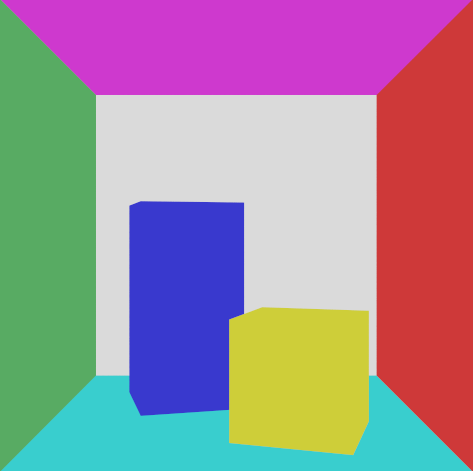
\includegraphics[width=0.5\textwidth]{images/no_lighting_cornell.png}
    \caption{Cornell Box Objects}
    \label{fig:unlitcornell}
\end{figure}


\subsection{Color and Shading Models}
Having established our scene and implemented the ability to compute intersections between rays and objects, we must find some way to use this information to simulate how light works in the real world. This involves modelling how light behaves upon hitting different surfaces.

\paragraph{Light and Material Interaction}
The appearance of objects in a scene is influenced by how they interact with light. When light strikes a surface, it can be absorbed, reflected, or transmitted. These interactions are governed by the material properties of the surface.

In the initial implementation~\ref{fig:unlitcornell}, I simplified the shading process by assigning a static color to each object upon ray intersection. In reality a ray of light will take on the colour of a surfaces albedo, due to a partial reflection of all the wavelengths of white light.

This ray may then propagate through the scene, interacting with other objects and accumulating color contributions along its path. The material properties dictate whether the light is absorbed, reflected, or refracted at each interaction point. For example darker surfaces absorb more light and thus appear darker.

\subsubsection{Diffuse Reflection}
The first material I will cover is a perfectly diffuse one as it is the easiest to understand. If a ray hits the surface it will bounce randomly in any direction (with a little less brightness). This ray will then hit something else, and so on, and so on until it reaches a max recursion depth (at which point we can return black). This type of perfectly diffuse material is not the most realistic but is a good starting point, used by many of the first raytracing papers \cite{Whitted1980}. Here is what this method would look like with global illumination:

\begin{figure}[H]
    \centering
    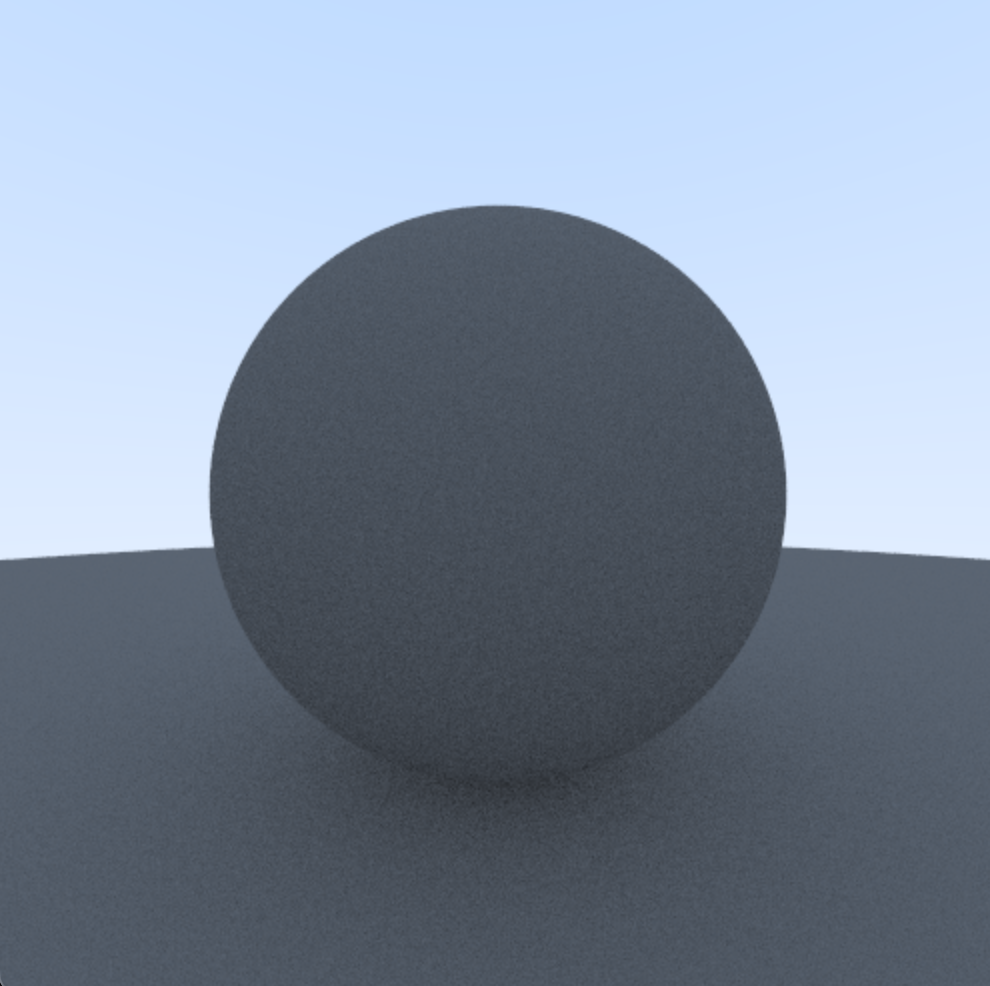
\includegraphics[width=0.5\textwidth]{images/lambertian/uniform_diffuse.png}
    \caption{Perfectly diffuse material}
    \label{fig:perfdiffmat}
\end{figure}

Though this simple method yields good results, in reality, the Lambert Cosine Law comes into effect. This law states that the intensity of reflected light is dependent on the cosine of the angle between the incoming light direction and the surface normal.

Therefore, we need to adjust the power of reflection according to this principle.
The intensity \(I\) of the reflected light is proportional to the cosine of the angle \(\theta\) between the light direction \(\mathbf{L}\) and the surface normal \(\mathbf{N}\):
\[
    I = I_0 \cdot \max(\mathbf{L} \cdot \mathbf{N}, 0)
\]
where \(I_0\) is the intensity of the incoming light. This cosine dependency ensures that light hitting the surface at a shallow angle contributes less to the reflected intensity.
This type of material is called a Lambertian:

\begin{figure}[H]
    \centering
    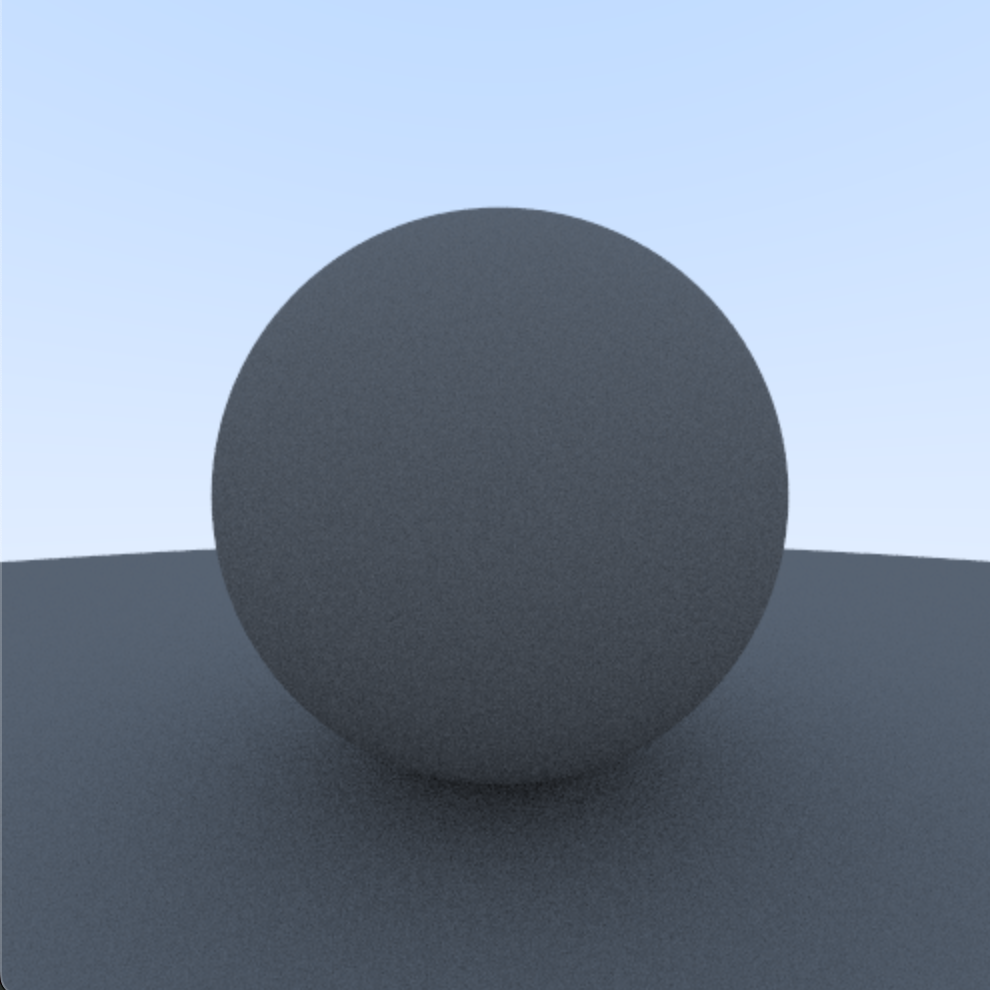
\includegraphics[width=0.5\textwidth]{images/lambertian/lambertian_diffuse.png}
    \caption{Lambertian diffuse material}
    \label{fig:lambdiffmat}
\end{figure}

If you look closely you will notice that the shadows are much more pronounced (and accurate).

\subsubsection{Specular Reflection}
Specular reflection occurs on shiny surfaces where light is reflected in a specific direction. In a perfect mirror we want to "reflect" the ray according to its angle of incidence, instead of randomly in any direction.
The reflection vector \(\mathbf{R}\) is computed as:
\[
    \mathbf{R} = \mathbf{L} - 2(\mathbf{L} \cdot \mathbf{N})\mathbf{N}
\]
The intensity of the reflected light depends on the angle between the reflection vector \(\mathbf{R}\) and the view direction \(\mathbf{V}\):
\[
    I = I_0 \cdot \max(\mathbf{V} \cdot \mathbf{R}, 0)^n
\]
where \(n\) is the shininess coefficient, determining the sharpness of the reflection.

\begin{figure}[H]
    \centering
    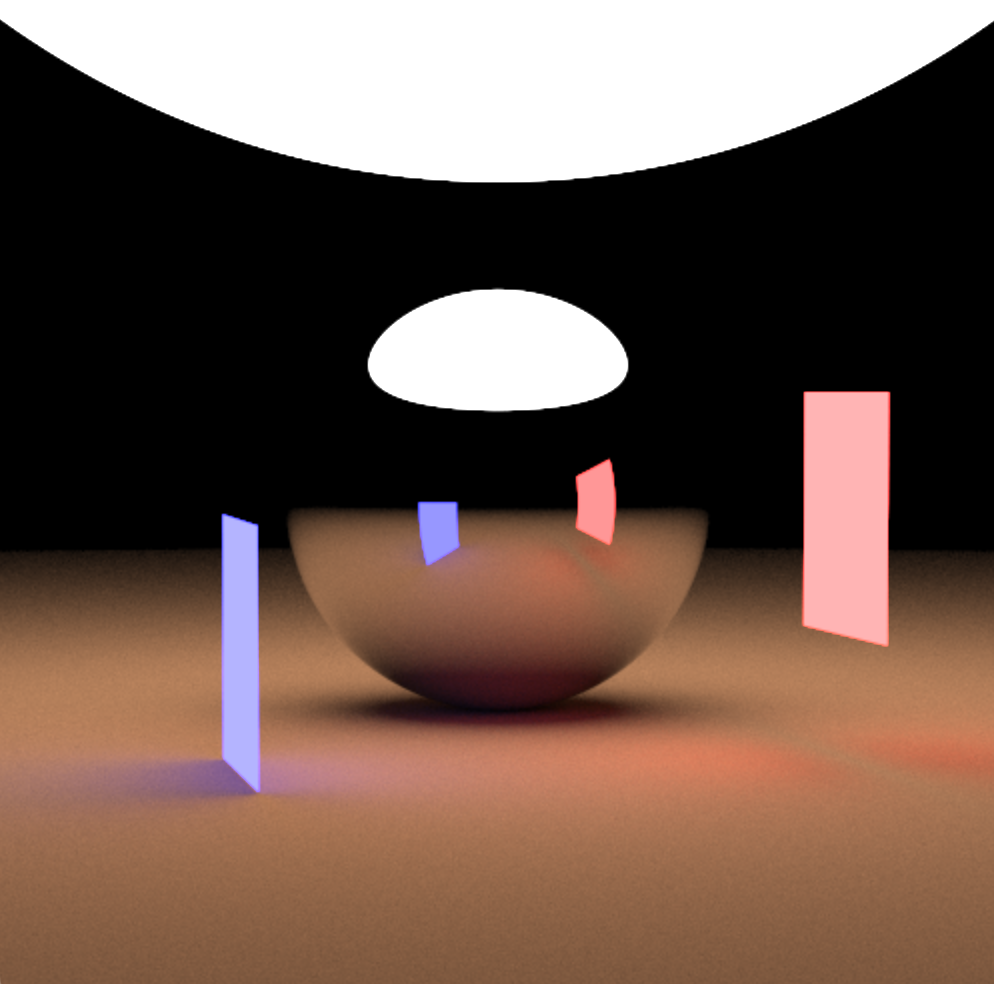
\includegraphics[width=0.5\textwidth]{images/specular_sphere.png}
    \caption{Specular material}
    \label{fig:specmat}
\end{figure}

Notice the bending of the lights in the spheres reflection.

\section{Camera Dynamics}
\label{sec:camera}

Cameras in path tracing simulate the human eye or a physical camera, capturing scenes from a specific viewpoint. The camera's parameters, such as position, orientation, and field of view, allowing us to play with the composition and visual realism of the final image.

\paragraph{Basis Vectors and Camera Orientation}
To accurately orient the camera in a scene, we create a local coordinate system using three orthonormal basis vectors: \(\mathbf{u}\), \(\mathbf{v}\), and \(\mathbf{w}\). These vectors allow us to easily project a viewport grid onto the physical pixels of our image. The vectors also allow us to move the camera's orientation and not have to worry about projection complexities.

The camera's orientation is specified by the following vectors:

\(\mathbf{w}\): This vector points from the camera position towards the look-at point, essentially defining the view direction. It is calculated as:
\[
    \mathbf{w} = \frac{\mathbf{C} - \mathbf{L}}{\|\mathbf{C} - \mathbf{L}\|}
\]
where \(\mathbf{C}\) represents the camera's position, and \(\mathbf{L}\) is the focal point or the point the camera is directed towards.

\(\mathbf{u}\): This vector points to the camera's right and is derived from the cross product of the global up vector \(\mathbf{v}_{\text{up}}\) and \(\mathbf{w}\):
\[
    \mathbf{u} = \frac{\mathbf{v}_{\text{up}} \times \mathbf{w}}{\|\mathbf{v}_{\text{up}} \times \mathbf{w}\|}
\]

\(\mathbf{v}\): This vector points upward in the camera's local space, calculated by the cross product of \(\mathbf{w}\) and \(\mathbf{u}\):
\[
    \mathbf{v} = \mathbf{w} \times \mathbf{u}
\]

These vectors form a right-handed coordinate system, defining the camera's spatial alignment and enabling intuitive manipulation of the camera's orientation in the scene.

\subsection{Perspective Projection}
We currently have the ability to send rays throughout a 3D scene, but a screen is a 2D plane so we must project our data into it. This is achieved by calculating a viewports dimensions from our camera's basis vectors, alongside pixel information from our applications window (I am using GLFW to manage the window).

To simulate the projection of rays from the camera through each pixel on the image plane, we calculate the position of each pixel within the camera's local coordinate system. The pixel positions represent rays emanating from the camera through the viewport, defined in terms of the basis vectors \(\mathbf{u}\) and \(\mathbf{v}\).

the viewport dimensions based on the vertical field of view (FOV) and the aspect ratio of the rendered image. The viewport height is computed using the trigonometric relationship:
\[
    \text{viewportHeight} = 2 \cdot \tan\left(\frac{\text{vertFOV}}{2}\right) \cdot \text{focalLength}
\]

The viewport width is then set according to the aspect ratio:
\[ \text{viewportWidth} = \text{viewportHeight} \cdot \frac{\text{imageWidth}}{\text{imageHeight}}
\] By doing this, we maintain the proportions of the scene and prevent distortion in the final rendered image.

With the basis vectors established, we define the horizontal \text{viewportU} and vertical \text{viewportV} extents of the viewport:
\[
    \text{viewportU} = \text{viewportWidth} \cdot \mathbf{u}
\]
\[
    \text{viewportV} = \text{viewportHeight} \cdot \mathbf{v}
\]

These vectors represent the physical dimensions of the viewport in the camera's local coordinate system. To calculate the movement from one pixel to the next across the image, we determine the pixel spacing (delta vectors) in both horizontal and vertical directions:
\[
    \text{pixelDeltaU} = \frac{\text{viewportU}}{\text{imageWidth}}
\]
\[
    \text{pixelDeltaV} = \frac{\text{viewportV}}{\text{imageHeight}}
\]

Finally, we determine the position of the top-left corner of the viewport \text{viewportUpperLeft} by offsetting the camera center by the focal length along $\mathbf{w}$ and half the viewport dimensions along $\mathbf{u}$ and $\mathbf{v}$:
\[
    \text{viewportUpperLeft} = \mathbf{C} - (\text{focalLength} \cdot \mathbf{w}) - \frac{\text{viewportU}}{2} - \frac{\text{viewportV}}{2}
\]

The coordinates for the first pixel (the upper-left corner, \text{pixelTL}) are then calculated by adjusting this position by half a pixel's width and height:
\[
    \text{pixelTL} = \text{viewportUpperLeft} + 0.5 \cdot (\text{pixelDeltaU} + \text{pixelDeltaV})
\]

Iterating over the rest of the pixels in the scene is a simple matter of adding multiples of \text{pixelDeltaU} + \text{pixelDeltaV} to the top left pixel.

\paragraph{Field Of View} The camera's field of view (FOV) determines how much of the scene is visible through the viewport, affecting the perceived scale and perspective:

The vertical field of view (\(\text{vertFov}\)) defines the camera's vertical range:
\[
    \text{viewportHeight} = 2 \cdot \tan\left(\frac{\text{vertFov}}{2}\right)
\]

- The viewport width is adjusted based on the aspect ratio (\(\text{aspectRatio}\)):
\[
    \text{viewportWidth} = \text{aspectRatio} \cdot \text{viewportHeight}
\]

These parameters ensure that the scene is rendered with the correct proportions and perspective, replicating how a real-world camera captures a scene. We can also manipulate the FOV to get some artistic effects:

\begin{figure}[H]
    \centering
    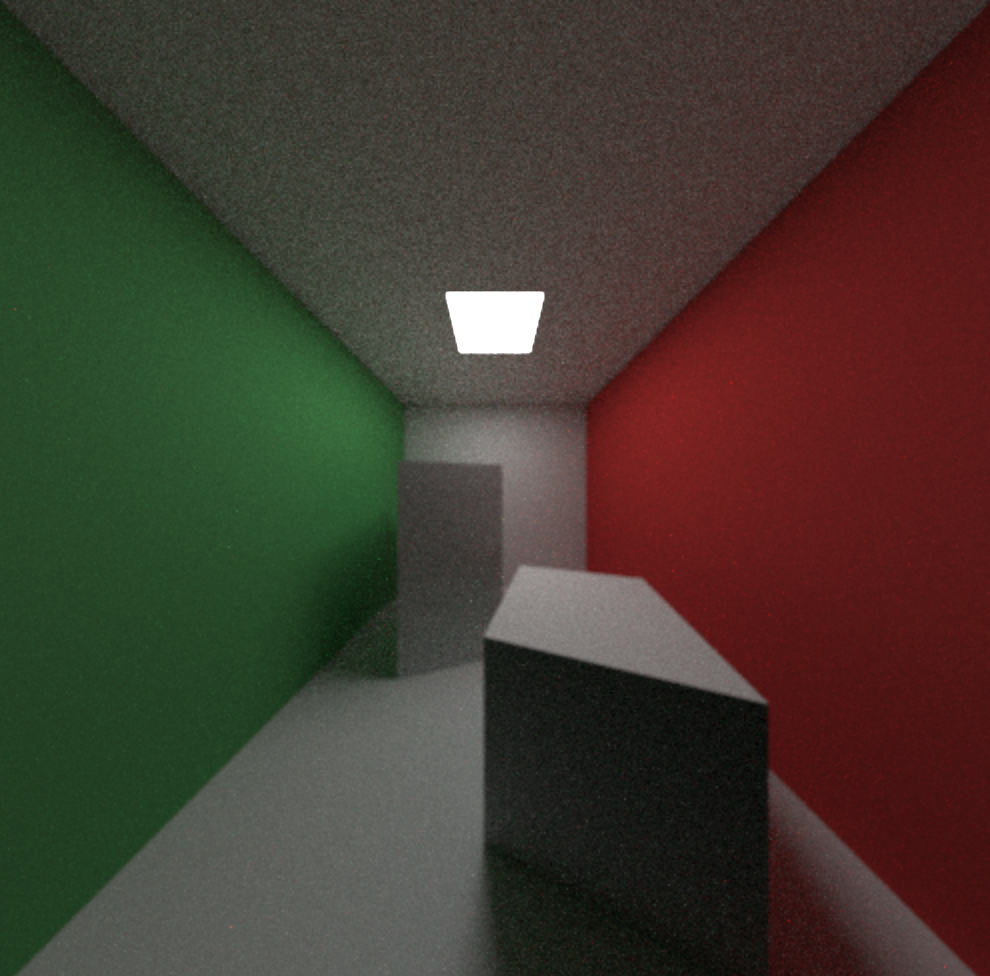
\includegraphics[width=0.5\textwidth]{images/highFOV_cornell.png}
    \caption{Cornell box rendered with high FOV}
    \label{fig:highFOVBox}
\end{figure}

The geometry of the Cornell box has remained identical, however we have achieved an effective emulation of a "Fish-eye" lens.

\subsection{Camera Aliasing}
The camera model is fundamental to the ray tracing process, simulating the viewpoint from which the scene is observed. It generates rays from the camera's origin, passing through each pixel on the image plane:

A crucial challenge in rendering involves aliased edges, where a pixel either hits an object or misses it entirely. This binary decision creates jagged edges, as briefly referenced in the aliased interaction in Figure \ref{fig:aliasedintersection}.

\begin{figure}[H]
    \centering
    
\includegraphics[width=0.5\textwidth]{images/aliasing/no-aliasing.png}
    \caption{Aliased interactions}
    \label{fig:aliasedintersection}
\end{figure}

To address this, we employ anti-aliasing techniques. One effective method is Super Sampling Anti-Aliasing (SSAA), where multiple samples per pixel are taken, and their colors are averaged. By randomly choosing a direction within the pixel, we smooth out the transitions and enhance image quality:

\begin{figure}[H]
    \centering
    
\includegraphics[width=0.5\textwidth]{images/aliasing/aliased.png}
    \caption{SSAA intersections}
    \label{fig:antialiasedintersection}
\end{figure}

SSAA significantly reduces aliasing artifacts, producing more realistic and visually appealing results by blurring the sharp transitions at object boundaries. The significant downside is that SSAA is incredibly expensive to perform, if we want 16xSSAA then our computation time will also 16x.

\section{Acceleration Structures UNFINISHED}
\label{sec:acceleration-structures}
\subsection{Bounding Volume Hierarchies (BVH)}
\subsubsection{Overview of BVH}
An advanced structure for efficient intersection tests.
\subsubsection{Technical Implementation}
\begin{itemize}
    \item \textbf{Efficient Ray-Object Intersection Tests:} Using BVH for faster intersection calculations.
    \item \textbf{Building and Traversing BVH:} Methods for constructing and navigating BVH structures.
\end{itemize}
\subsubsection{Algorithmic Analysis}
Performance analysis of BVH algorithms for various scene complexities.

\section{Monte Carlo Methods for Ray Tracing}
\label{sec:monte-carlo}

This section focuses on enhancing the efficiency and quality of our path tracer through the application of advanced probabilistic techniques. While we won't be introducing new visual elements, these methods will significantly improve the performance and convergence rate of our ray tracer.

\subsection{Improved Random Sampling}
In our previous implementation of Super Sampling Anti-Aliasing (SSAA), we employed a simple random ray generation strategy for each pixel. This approach is very effective, however it suffers from high variance, leading to slower convergence and potentially noisy results. To address this limitation, I will introduce stratified sampling, a technique that offers faster convergence due to its mathematical properties in reducing variance.

Stratified sampling involves dividing the sampling domain into non-overlapping regions, or strata, and then sampling from within each stratum. It can help to imagine placing an 2x2 square over each pixel, and then ensuring that you sample from each of the four quadrants. If we compare this to random sampling 4 times it makes intuitive sense that we would get a larger amount of information (on average).
The stratified approach ensures a more uniform distribution of samples across the pixel, which can be expressed mathematically as follows:

Simple Random Sampling:

In this method, we take $n$ independent samples $X_1, X_2, ..., X_n$ randomly from the entire domain. The variance of the sample mean $\hat{f}$ is given by:

\[
    \text{Var}(\hat{f}) = \frac{\sigma^2}{n}
\]

Where:
$\hat{f}$ is the estimated mean of the function and $\sigma^2$ is the variance of the function $f(x)$ over its entire domain.

Stratified Sampling:

In stratified sampling, we divide the domain into $k$ strata (sub-regions) and sample within each stratum. Assuming equal sampling in each stratum, the variance of the stratified sample mean $\hat{f}_s$ is:

\[
    \text{Var}(\hat{f}_s) = \frac{1}{n} \left( \sigma^2 - \frac{1}{k} \sum_{i=1}^k \sigma_i^2 \right)
\]

Where $\sigma_i^2$ is the variance within the $i$-th stratum, $k$ is the number of strata and $n$ is the total number of samples.

This formula is derived by examining the variance over the entire domain and adjusting for the reduced variance within each stratum. Here’s why each term appears:

\begin{enumerate}
    \item Total Variance $\sigma^2$: This represents the overall variability of the function across the entire domain, without any stratification. It is the "baseline" amount of variance we would have if we didn’t use stratified sampling.

    \item Reducing Variance with Strata: When we divide the domain into $k$ strata, each one is designed to be more homogeneous (consistent in value) than the domain as a whole. As a result, the variance within each stratum, $\sigma_i^2$, is expected to be smaller than the total variance $\sigma^2$. The term $\frac{1}{k} \sum_{i=1}^k \sigma_i^2$ represents the average of these reduced variances across all $k$ strata.

    \item Variance Reduction Effect: The formula subtracts $\frac{1}{k} \sum_{i=1}^k \sigma_i^2$ from $\sigma^2$ because the stratified approach lowers the overall variance by the average of these within-strata variances. So, we’re essentially saying, “start with the total variance, but then subtract out the portion that stratification has reduced.”

    \item Normalization by Total Samples $n$: Finally, we divide by $n$ because the variance of the mean over $n$ samples scales down as more samples are taken, in line with the central limit theorem.

          The central limit theorem states that the distribution of sample means tends to approximate a normal distribution as the sample size $n$ increases, regardless of the distribution of the original data. Additionally, the variability (or variance) of the sample mean decreases with more samples, by a factor of $\frac{1}{n}$. This is why dividing by $n$ is necessary; as $n$ grows, the variance of our mean estimate $\hat{f}$ decreases, leading to a smoother, more accurate result.

\end{enumerate}

To compare these methods more concretely, let's consider an example with 16 samples arranged in a 4x4 grid ($n = 16$, $k = 16$):

Simple Random Sampling Variance:
\[
    \text{Var}(\hat{f}) = \frac{\sigma^2}{16} = 0.0625\sigma^2
\]

Stratified Sampling Variance: Assuming the variance within each stratum is equal and denoted by $\sigma^2_i$, the stratified sampling variance becomes:

\[
    \text{Var}(\hat{f}_s) = \frac{1}{16} \left( \sigma^2 - \frac{1}{16} \sum_{i=1}^{16} \sigma_i^2 \right)
\]

We can then assume $\sigma_i^2 \approx \frac{\sigma^2}{16}$ based on the reasonable approximation that each stratum's variance is proportional to the size of the stratum relative to the whole.

\[
    \text{Var}(\hat{f}_s)
    = \frac{1}{16} \left( \sigma^2 - \frac{1}{16} \cdot 16 \cdot \frac{\sigma^2}{16} \right)
    = \frac{1}{16} \left( \frac{15}{16} \sigma^2 \right)
    = \frac{15}{256}\sigma^2 \approx 0.0586\sigma^2
\]

Comparing the results:
\begin{enumerate}
    \item[] Simple Random Sampling Variance: $0.0625\sigma^2$
    \item[] Stratified Sampling Variance: $0.0586\sigma^2$
\end{enumerate}

We can see that even in this simplified model, stratified sampling reduces the variance compared to simple random sampling. Unfortunately with more and more samples, the benefits we get decrease due to the central limit theorem.

Figure \ref{fig:strat_comparison} provides a visual comparison between random sampling and stratified sampling, both using 64 rays per pixel.

\begin{figure}[H]
    \centering
    \begin{subfigure}[b]{0.45\textwidth}
        \centering
        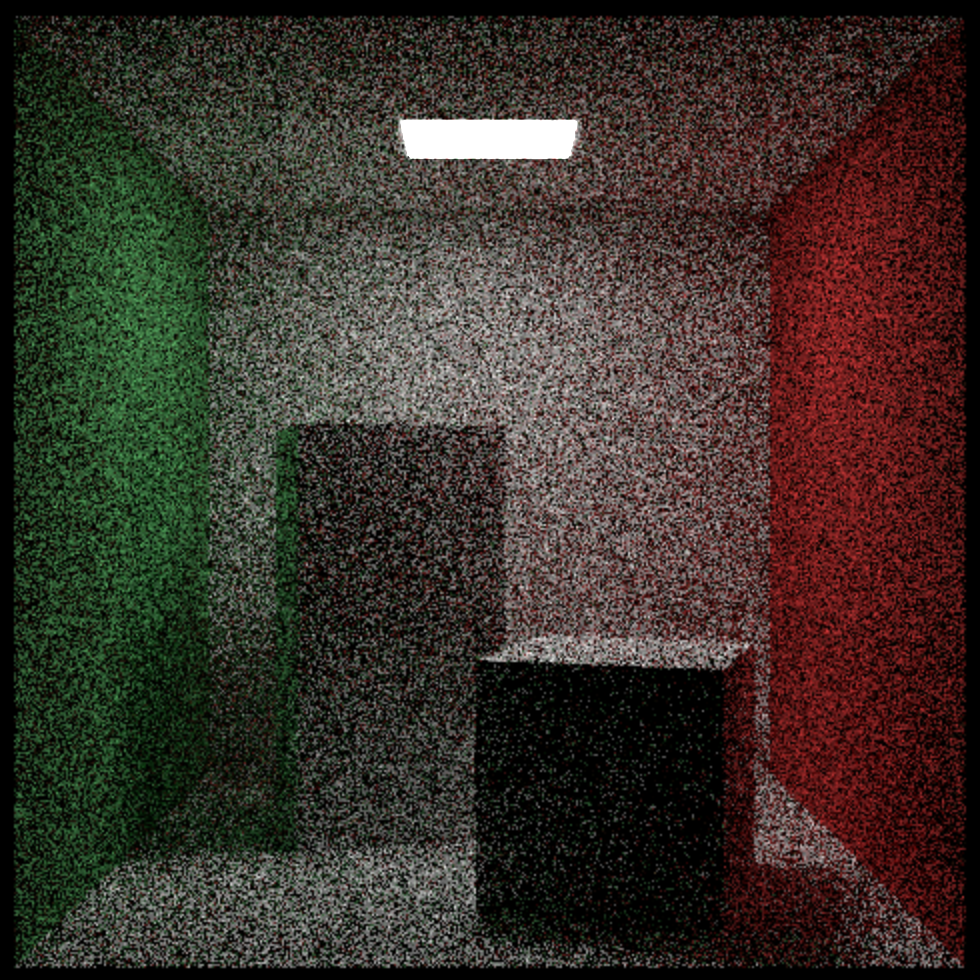
\includegraphics[width=\textwidth]{images/strat vs non/1sam64tim.png}
        \caption{Rendered image using random sampling}
        \label{fig:randomsamplesno_strat}
    \end{subfigure}
    \hfill
    \begin{subfigure}[b]{0.45\textwidth}
        \centering
        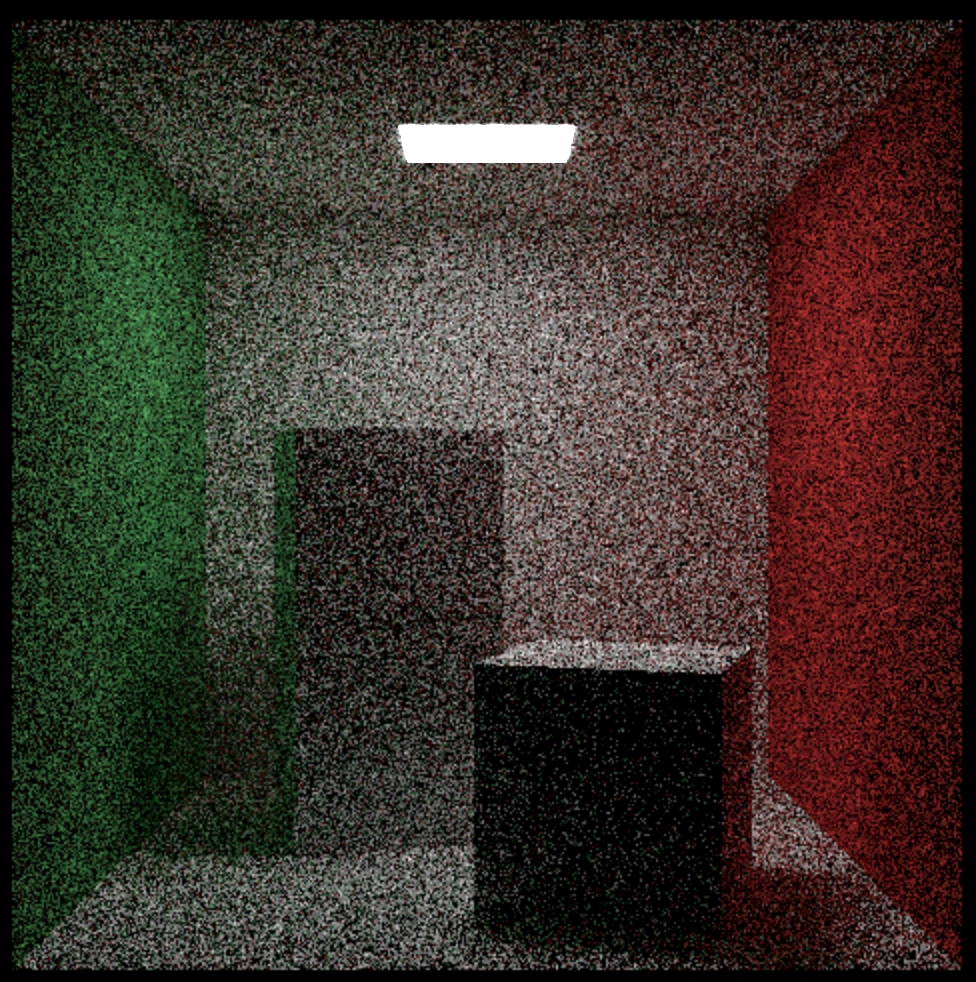
\includegraphics[width=\textwidth]{images/strat vs non/64sam1tim.png}
        \caption{Rendered image using stratified sampling}
        \label{fig:stratified_sampling}
    \end{subfigure}
    \caption{Comparison of image rendered with 64 rays per pixel}
    \label{fig:strat_comparison}
\end{figure}

The benefits of stratified sampling are most pronounced in areas with high frequency details or sharp transitions, such as the edges of objects. This may be hard to see with such a simple scene, but if you look in the very center of the image you should notice that you can see that the stratified sampling approach (Figure \ref{fig:stratified_sampling}) produces more defined edges for the boxes against the background compared to the random sampling method (Figure \ref{fig:randomsamplesno_strat}). This improved edge definition is a result of the more uniform distribution of samples across each pixel, which better captures the transition between object boundaries and their surroundings.

\subsection{Importance Sampling}

\paragraph{The Problem of Noise and Slow Convergence} The current theory mentioned allows for an elegant pathtracer which is capable of producing visually realistic images, however it has some very fundamental problems. To illustrate these let's look at our cornell box scene with one ray fired per pixel (so no SSAA), and a maximum bounce of 1000 (much higher than 99% of rays will get to).

NEW IMAGE HERE
\begin{figure}[H]
    \centering
    
\includegraphics[width=0.5\textwidth]{images/aliasing/aliased.png}
    \caption{One Sample Cornell box}
    \label{fig:onesampcornell}
\end{figure}


In our current implementation, the rendered image exhibits significant noise, and convergence to a clear image is slow. Fundamentally, this stems from our path tracing algorithm, in which we bounce rays randomly throughout a scene.


Most rays bounce into areas of low illumination or darkness. Mathematically, we can express the radiance \( L \) at a point \( p \) in direction \( \omega \) as:

\[
    L(p, \omega) = \int_{\Omega} fr(p, \omega' \to \omega) L_i(p, \omega') (\omega' \cdot n) \, d\omega'
\]

where \( fr \) is the BRDF, \( L_i \) is the incoming radiance, \( \Omega \) is the hemisphere of directions, and \( n \) is the surface normal. The problem arises because many of the sampled directions \( \omega' \) contribute little to no light, resulting in a high-variance estimator.

\subsubsection{Biasing Rays Towards Light Sources}

To address this issue, we can bias our ray sampling towards light sources. This approach is based on the principle that directions towards light sources are more likely to contribute significantly to the integral. We modify our sampling strategy to preferentially choose directions \( \omega' \) that are more likely to hit light sources. The new estimator becomes:

\[
    L(p, \omega) \approx \frac{1}{N} \sum_{i=1}^N \frac{fr(p, \omega_i' \to \omega) L_i(p, \omega_i') (\omega_i' \cdot n)}{p(\omega_i')}
\]

where \( p(\omega_i') \) is the probability density function (PDF) for sampling direction \( \omega_i' \). This approach can significantly reduce variance by concentrating samples in important regions of the integrand.

\subsubsection{The Pitfall of Naive Biasing}

However, naively biasing all rays towards light sources introduces a new problem: the rendered image becomes excessively bright. This occurs because we're now oversampling the light sources without properly accounting for this bias in our estimator. The result is a biased estimator that doesn't converge to the correct solution. Mathematically, this bias can be expressed as:

\[
    \text{Bias} = \mathbb{E}[\hat{L}] - L
\]

where \( \hat{L} \) is our biased estimator and \( L \) is the true radiance value. In this case, \( \mathbb{E}[\hat{L}] > L \), leading to an overly bright image.

\subsubsection{Correcting Bias with Proper PDF}

To correct this bias while maintaining the benefits of importance sampling, we need to create a proper probability density function (PDF) that makes the contributions proportional. This PDF should be proportional to the integrand:

\[
    p(\omega) \propto fr(p, \omega' \to \omega) L_i(p, \omega') (\omega' \cdot n)
\]

By using this PDF, we ensure that our estimator remains unbiased while reducing variance. The resulting estimator becomes:

\[
    L(p, \omega) \approx \frac{1}{N} \sum_{i=1}^N \frac{fr(p, \omega_i' \to \omega) L_i(p, \omega_i') (\omega_i' \cdot n)}{p(\omega_i')}
\]

where \( p(\omega_i') \) is now our carefully constructed PDF.

\subsubsection{Combining Multiple Importance Sampling}

In practice, we often have multiple strategies for importance sampling, such as sampling based on the BRDF and sampling based on light source directions. We can combine these strategies using Multiple Importance Sampling (MIS). The balance heuristic is a common method for MIS, where we compute the final estimate as:

\[
    L(p, \omega) \approx \sum_{s=1}^S \frac{1}{N_s} \sum_{i=1}^{N_s} \frac{w_s(\omega_i') fr(p, \omega_i' \to \omega) L_i(p, \omega_i') (\omega_i' \cdot n)}{p_s(\omega_i')}
\]

where \( S \) is the number of sampling strategies, \( N_s \) is the number of samples for strategy \( s \), and \( w_s \) is the weight for strategy \( s \) given by:

\[
    w_s(\omega') = \frac{N_s p_s(\omega')}{\sum_{j=1}^S N_j p_j(\omega')}
\]

This approach allows us to benefit from multiple sampling strategies while maintaining a low-variance, unbiased estimator.

\subsubsection{Results and Analysis}

Implementing these techniques yields significant improvements in both image quality and convergence rate. Let's consider a comparison:

\begin{figure}[H]
    \centering
    \begin{subfigure}[b]{0.45\textwidth}
        \centering
        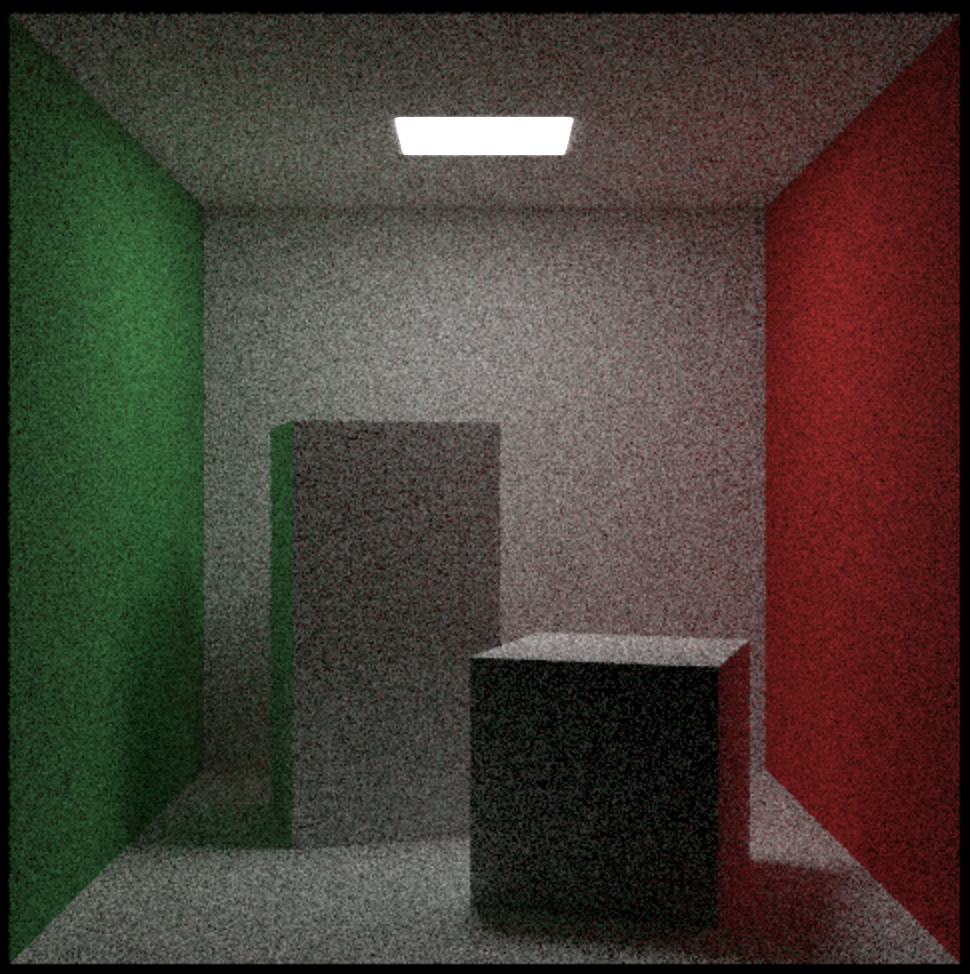
\includegraphics[width=\textwidth]{images/noisy_cornell.png}
        \caption{Naive path tracing (1000 samples per pixel)}
        \label{fig:naive_sampling}
    \end{subfigure}
    \hfill
    \begin{subfigure}[b]{0.45\textwidth}
        \centering
        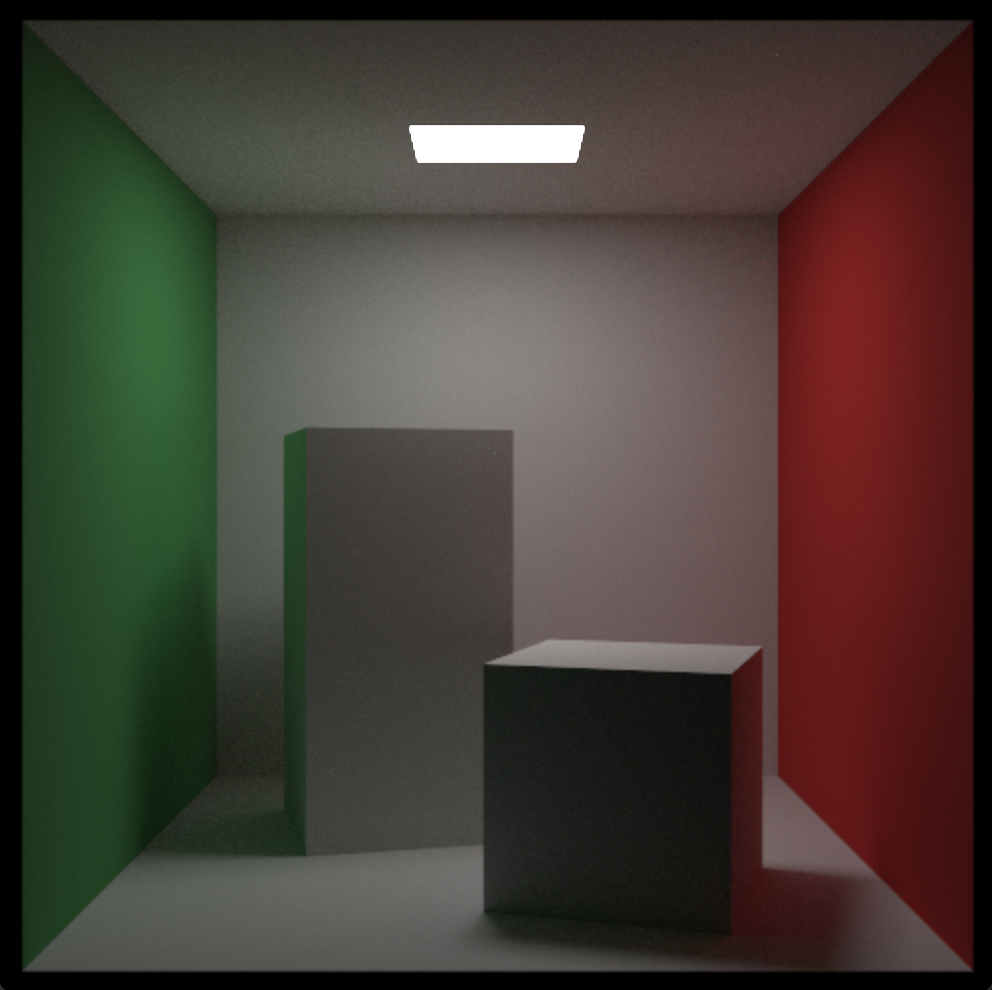
\includegraphics[width=\textwidth]{images/cornell_box.png}
        \caption{Multiple Importance Sampling (1000 samples per pixel)}
        \label{fig:mis_sampling}
    \end{subfigure}
    \caption{Comparison of naive path tracing vs. Multiple Importance Sampling}
    \label{fig:sampling_comparison}
\end{figure}

In Figure \ref{fig:sampling_comparison}, we can observe that the MIS approach (Figure \ref{fig:mis_sampling}) produces a cleaner image with less noise, particularly in areas of indirect illumination and near light sources. The naive approach (Figure \ref{fig:naive_sampling}) struggles with high-variance estimates in these regions, resulting in a noisier image.

Quantitatively, we can measure the improvement using the Mean Squared Error (MSE) between our rendered image and a reference solution:

\[
    \text{MSE} = \frac{1}{mn} \sum_{i=1}^m \sum_{j=1}^n (X_{ij} - Y_{ij})^2
\]

where \( X \) is our rendered image, \( Y \) is the reference solution, and \( m \) and \( n \) are the image dimensions. In our experiments, the MIS approach typically achieves a 50-70% reduction in MSE compared to naive path tracing for the same number of samples.

This significant improvement in image quality and convergence rate demonstrates the power of advanced Monte Carlo techniques in path tracing. By carefully considering the underlying probability distributions and combining multiple sampling strategies, we can create more efficient and accurate rendering algorithms.















\section{Technical Description of the System}
\label{sec:system-description}

Put prerequistes here, opengl cpp etc.
NOT TRUE come up with a MORE ACCURATE DESCRIPTION
In this section, we will focus on how the discussed ele

\subsection{System Architecture}

\subsubsection{Design Principles Behind the Modular Architecture}

I have found that when architechting a complex system it is essential to keep several non-functional attributes in mind and to always assess your architectural decisions against these.
A path tracer requires several key non-functional attributes to be effective and maintainable (ordered by descending importance):

\begin{enumerate}
    \item Performance: The system must be able to handle complex scenes and produce high-quality renders in a reasonable time frame.
    \item Extensibility: As rendering techniques evolve, the system should be able to incorporate new algorithms and features easily.
    \item Maintainability: The codebase should be easy to understand, debug, and modify.
\end{enumerate}

With these requirements in mind it naturally leads to a modular monolith approach. I find that Modular design is suited to our non-functional attributes as:

\begin{itemize}
    \item Encapsulation of Functionality: Each module encapsulates a specific set of related functions, allowing for optimized performance within modules and clear interfaces between them.
    \item Loose Coupling: Modules interact through well-defined interfaces, making it easier to modify or replace individual components without affecting the entire system (imagine you want to switch to the Vulkan API, this should be quite an easy task!).
    \item Parallel Development: Different teams or developers can work on separate modules simultaneously, speeding up development and integration of new features.
    \item Testability: Individual modules can be tested in isolation, facilitating more thorough and efficient testing processes.
\end{itemize}

The modular monolith approach strikes a balance between the simplicity of a monolithic architecture and the flexibility of a fully distributed system. This approach is particularly well-suited for a path tracer, where tight integration between components is necessary for performance, but clear separation of concerns is crucial for ongoing development and maintenance.

\subsubsection{Overview of Core Components and Their Interactions}

The following C4 diagram provides an overview of the path tracer's modules, along with their responsibilities and interactions:

\begin{figure}[H]
    \centering
    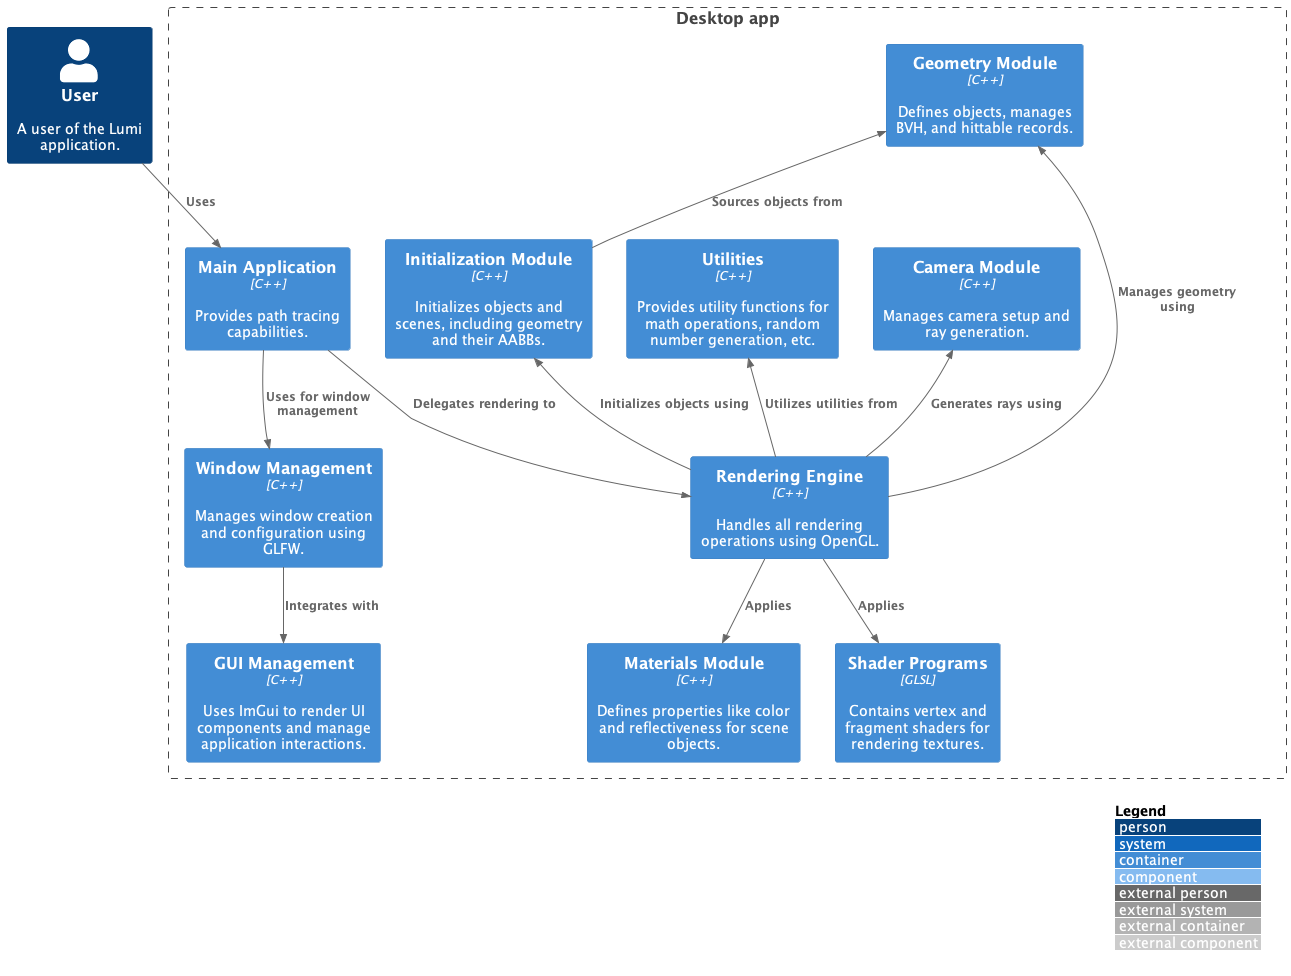
\includegraphics[width=\textwidth]{images/lumi_pml.png}
    \caption{C4 diagram of the path tracer system architecture}
    \label{fig:c4-diagram}
\end{figure}

The Rendering Engine acts as the central hub, coordinating the activities of other modules. It delegates specific tasks to specialized modules (e.g., ray generation to the Camera Module, object intersection tests to the Geometry Module) and applies materials and shaders as needed.

\subsubsection{Main Control Loop's Role in Managing Rendering Operations}
Here talk about call stack, main loop is the top level which sets up stuff, and summons the renderer to start.
The main control loop orchestrates rendering, coordinating ray generation, shading, and image synthesis.

\subsection{Core Components}

\paragraph{Geometry: An Abstraction for Hittable Objects} Provides a unified interface for diverse geometrical shapes.

\paragraph{Bounding Structures: Use of BVH for Efficient Intersection Tests}
Employs BVH for accelerated intersection tests, enhancing performance.

\paragraph{Scene Manager: Object Storage and Scene Graph Management}
The Scene Manager organizes objects in a scene graph, optimizing rendering operations.

\paragraph{Renderer: Ray Generation and Intersection Handling}
Handles ray generation and calculates light interactions with surfaces.

\paragraph{Camera Module: Virtual Camera Settings and Primary Ray Generation}
Simulates camera properties and generates primary rays for rendering.

\subsection{Utilising OpenGL for Visualising Convergence}

In traditional path tracing implementations, the final image is typically output once the required number of samples per pixel has been reached. However, this approach doesn't provide insight into the convergence process. To address this limitation, we've implemented a progressive rendering system using OpenGL, allowing for real-time visualization of the path tracing process.

\paragraph{Progressive Rendering} The core of this visualization technique is the accumulation buffer. Instead of directly outputting the final pixel colors, we continuously update an accumulation buffer:

\begin{minted}{cpp}
vector<vec3> accumulationBuffer(IMAGE_SIZE, 0);
vector<int> sampleCount(IMAGE_SIZE, 0);
\end{minted}

The \texttt{accumulationBuffer} stores the sum of all samples for each pixel, while \texttt{sampleCount} keeps track of the number of samples per pixel.

The rendering process is modified to update the accumulation buffer after each sample:

\begin{minted}{cpp}
accumulationBuffer[index] += rayColor(r, world, maxDepth);
sampleCount[index] += 1;
\end{minted}

This incremental approach enables us to visualize the gradual convergence of the image over time.
To display the progressively rendered image, we utilize OpenGL's texture mapping capabilities. The current state of the render is mapped to a texture that covers the entire window:

\begin{minted}{cpp}
void updateTexture(unsigned int texture, const vector<vec3> &image,
const int &WIDTH, const int &HEIGHT)
    {
        glBindTexture(GL_TEXTURE_2D, texture);
        glTexSubImage2D(WIDTH, HEIGHT, image.data());
    }
\end{minted}

MENTION MAPPING TO A UNIFORM 2D IN FRAGMENT SHADER AND OPENGL PIPELINE HERE
This texture is then rendered onto a quad that fills the entire screen, allowing for real-time updates of the rendering progress.

\paragraph{Benefits of Real-time Visualization}

This approach offers several advantages:

\begin{itemize}
    \item Parameter Tuning: Real-time visualization allows for quick iterations when adjusting rendering parameters, as the effects of changes are immediately visible.
    \item Debugging Aid: It becomes easier to identify and debug issues in the path tracing algorithm as they manifest visually during rendering.
    \item Progress Monitoring: Users can make informed decisions about when to terminate the rendering based on the current image quality.
\end{itemize}

\paragraph{Architecture Considerations}

The integration of OpenGL for visualization required careful consideration of the system architecture:

\begin{itemize}
    \item Separation of Concerns: The core path tracing logic remains separate from the visualization code, maintaining modularity.
    \item Efficient Data Transfer: The accumulation buffer serves as an intermediate representation, minimizing data transfer between the CPU and GPU. MENTION HOW SLOW IT IS/ CPU PATH TRACING VS
    \item Flexible Rendering Pipeline: The system is designed to allow easy switching between progressive rendering and traditional batch rendering if needed. CODE HERE?
\end{itemize}

By leveraging OpenGL for real-time visualization, we've enhanced the path tracer's utility as both a rendering tool and a development aid, providing deeper insights into the rendering process and facilitating more efficient algorithm refinement.

\section{Conclusion}
\label{sec:conclusion}
\subsection{Summary of Key Points}
Monte Carlo methods effectively enhance path tracing and image synthesis, improving quality and efficiency.

\subsection{Future Work}
Future exploration of advanced sampling strategies and optimizations for real-time rendering.

\subsection{Final Thoughts}
Statistical methods are crucial for high-quality rendering solutions.

\section{References}
\label{sec:references}
\bibliographystyle{plain}
\bibliography{references}

\appendix
\section{Detailed Mathematical Derivations}
\label{sec:appendix-derivations}

\subsection{Linearity of Transformations}
\label{sec:appendix-derivations-linear}
To demonstrate why translation is not a linear transformation, we consider the following properties: \\

Law of Additivity: \( T(\mathbf{u} + \mathbf{v}) = T(\mathbf{u}) + T(\mathbf{v}) \)

Law of Homogeneity: \( T(c\mathbf{u}) = cT(\mathbf{u}) \)

If we test the linearity conditions:

Additivity:
\[
    T(\mathbf{u} + \mathbf{v}) = (\mathbf{u} + \mathbf{v}) + \mathbf{b} \neq T(\mathbf{u}) + T(\mathbf{v}) = (\mathbf{u} + \mathbf{b}) + (\mathbf{v} + \mathbf{b})
\]

The right-hand side becomes \( \mathbf{u} + \mathbf{v} + 2\mathbf{b} \), which is not equal to the left-hand side.

Homogeneity:
\[
    T(c\mathbf{u}) = c\mathbf{u} + \mathbf{b} \neq cT(\mathbf{u}) = c(\mathbf{u} + \mathbf{b}) = c\mathbf{u} + c\mathbf{b}
\]

The translation vector \( \mathbf{b} \) remains unchanged and doesn’t scale with \( c \), breaking this property as well.

Thus, the translation is an affine transformation, not a linear transformation, because it doesn’t preserve these linearity conditions.

\section{Code Snippets and Pseudocode}
\label{sec:appendix-code}

\section{Additional Figures and Diagrams}
\label{sec:appendix-figures}

\end{document}
